Single-cell sequencing has opened a window into the heterogeneity and dynamics of biology on a cellular scale. One prominent application is to study the dynamics of cell differentiation, development, and response to stimuli. Discoveries in this area have the potential to fuel advances in drug development and cell engineering, with impacts on fields such as regenerative medicine and immuno-oncology.

\begin{figure}
    \centering
    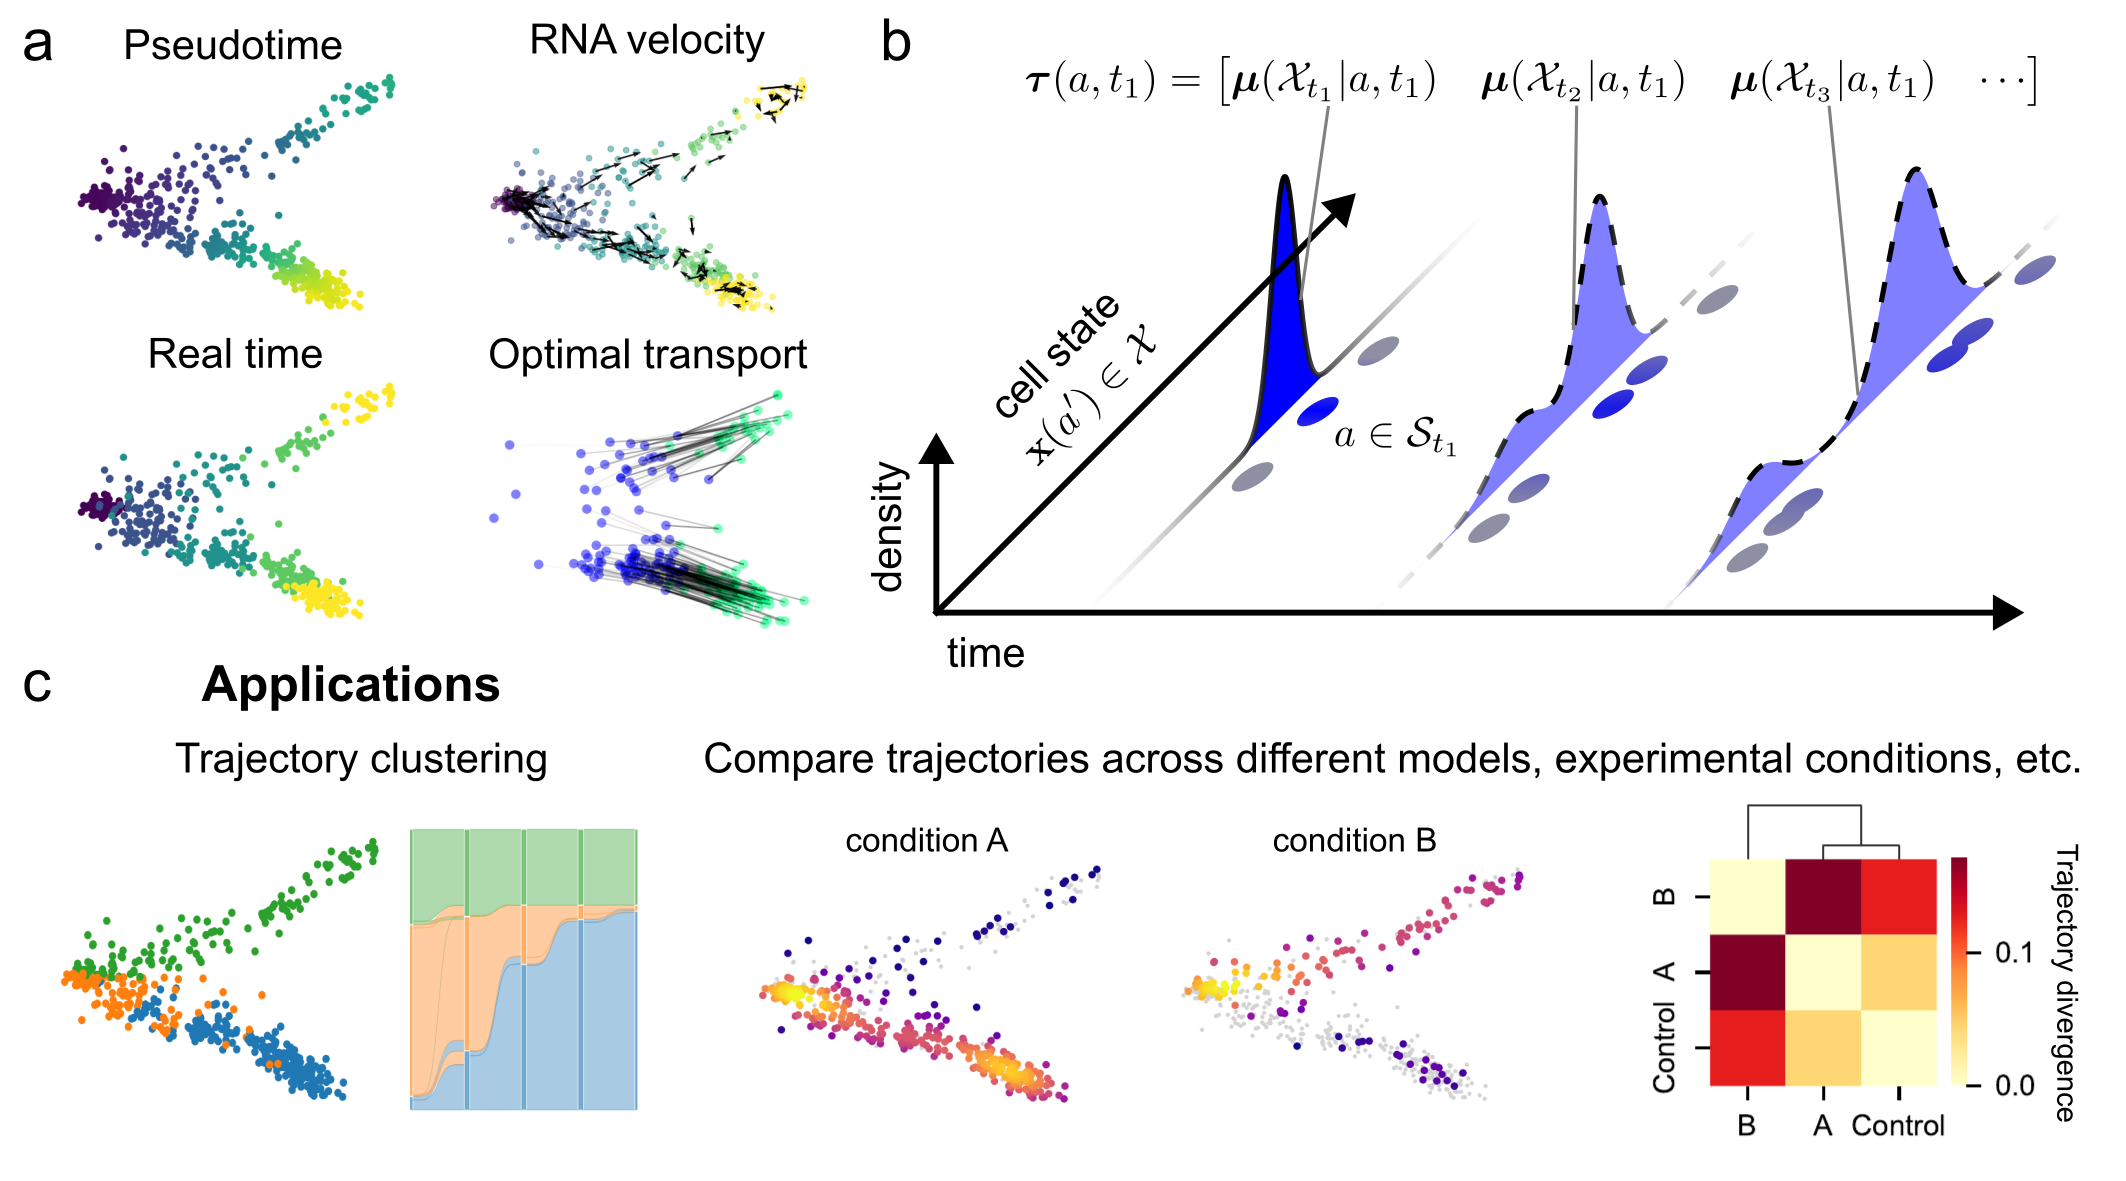
\includegraphics[width=\textwidth]{ch2/figs/Introduction_method_overview.png}
    \caption{
    Overview of real-time trajectory featurization method.
    (a) Visualization of pseudotime, RNA velocity, and optimal transport methods on a simulated dataset of cell differention under diffusion-drift dynamics.
    (b) Schematic illustrating concept of representing trajectories as a feature vector.
    (c) Applications of trajectory featurization, including clustering that respects the underlying trajectory model, and comparison of trajectories under distinct experimental conditions.
    }
    \label{fig:intro}
    \label{fig:intro-a}
    \label{fig:intro-b}
    \label{fig:intro-c}
\end{figure}

However, the destructive nature of single-cell sequencing makes it impossible to profile a cell at more than a single time point. This has led to the development of a variety of trajectory inference methods to study dynamic cellular processes. Some of the most frequently used tools attempt to order cells along a pseudotime axis based on the similarity of their gene expression \citep{haghverdiDiffusionPseudotimeRobustly2016}. While pseudotime methods have proven extremely useful for discovering transient states in differentiation \citep{laddachBranchingModelLineage2023}, they are limited in their ability to make falsifiable predictions \citep{weinrebFundamentalLimitsDynamic2018}. Many methods have sought to increase the resolution of inferred trajectories; for example, RNA velocity and related methods estimate the rate of change in cell state with respect to time by solving a system of mass balance equations using spliced versus unspliced transcripts \citep{lamannoRNAVelocitySingle2018}. However, there is some debate about the interpretability of inferred velocities \citep{gorinRNAVelocityUnraveled2022}, and it is difficult to find ground truths to assess their accuracy.

Another option is to incorporate time point information directly into the trajectory model. Such approaches predict trajectories for each cell by mapping cell distributions from one time point to another \citep{lavenantMathematicalTheoryTrajectory2021}. The mapping function is flexible and can be parameterized over discrete cell states, \citep{schiebingerOptimalTransportAnalysisSingleCell2019} or over the continuous underlying gene expression space \citep{tongTrajectoryNetDynamicOptimal2020}. In this work, we focus on discrete maps fit using optimal transport. In addition to predicting cell fates at single-cell resolution, real-time models are also able to model cell proliferation and death as functions of time \citep{schiebingerOptimalTransportAnalysisSingleCell2019}. Finally, the accuracy of real-time trajectory models can be evaluated by comparison to ground-truth trajectories, such as experiments incorporating cell-barcoding technologies for lineage tracing \citep{weinrebLineageTracingTranscriptional2020a}.

Despite the advantages of real-time trajectory inference methods, there are challenges in interpreting their predictions. Whereas trajectories in pseudotime models are defined by a small number of parameters (i.e. pseudotime estimate and branch identity), and velocity vectors can be projected onto a low-dimensional visualization, real-time trajectories are inherently high-dimensional (Fig~\ref{fig:intro-a}a). The outputs of real-time models may be visualized as fate probabilities for a group of target populations \citep{kleinMappingCellsTime2023a}, but this approach may not work if there is substantial heterogeneity in cell states at the target timepoint. For example, clusters may be highly correlated with time \citep{kurdEarlyPrecursorsMolecular2020}, rather than with the biological heterogeneity within each time point. Another challenge of real-time methods is that there is no established way to compare trajectory models fit on disjoint sets of cells. This problem arises when there are distinct experimental conditions that must be modeled separately. Previously, metrics like the Wasserstein distance have been used to compare model predictions to ground truths for each time point \citep{yeoGenerativeModelingSinglecell2021}, however this scales poorly with the size of the dataset. There exists a need to learn representations of real-time single-cell trajectories that facilitate downstream tasks, such clustering to identify distinct pathways of differentiation, and hypothesis testing to identify experimental conditions that significantly affect cell responses in time.

We propose a method that represents the state of a cell across the entirety of its trajectory as a single feature vector. This allows us to compare trajectories of cells that were observed at different time points, as well as to compare trajectories between different models, or disjoint experimental conditions. Our method works by first predicting a cell's ancestor and descendant distributions at each time point, and then embedding these distributions into a vector in a reproducing kernel Hilbert space (RKHS). We show that this information-rich featurization is useful for clustering cell fates, especially on highly heterogeneous datasets. Furthermore, we demonstrate how an intentional choice of kernel induces sensible distance metrics between trajectories, and explore its utility for quantifying time-dependent experimental perturbations. The proposed method is implemented for trajectory inference models utilizing optimal transport, however it has the potential to be adapted for any trajectory model which utilizes mappings between cell distributions at discrete time points.

